\documentclass[sigconf,anonymous]{aamas}

\usepackage{booktabs}
\usepackage{amsmath}
% amssymb omitted: the aamas class already provides it and reloading
% it redefines \Bbbk
\usepackage{amsthm}
\usepackage{balance}
\usepackage{tikz}
\usepackage{algorithm}
\usepackage{algpseudocode}

\newtheorem{proposition}{Proposition}
\newtheorem{corollary}[proposition]{Corollary}
\newtheorem{definition}{Definition}
\theoremstyle{remark}
\newtheorem{remark}{Remark}
\newtheorem{example}{Example}

%%% AAMAS-2027 copyright block (do not change!)
\makeatletter
\gdef\@copyrightpermission{
  \begin{minipage}{0.2\columnwidth}
   \href{https://creativecommons.org/licenses/by/4.0/}{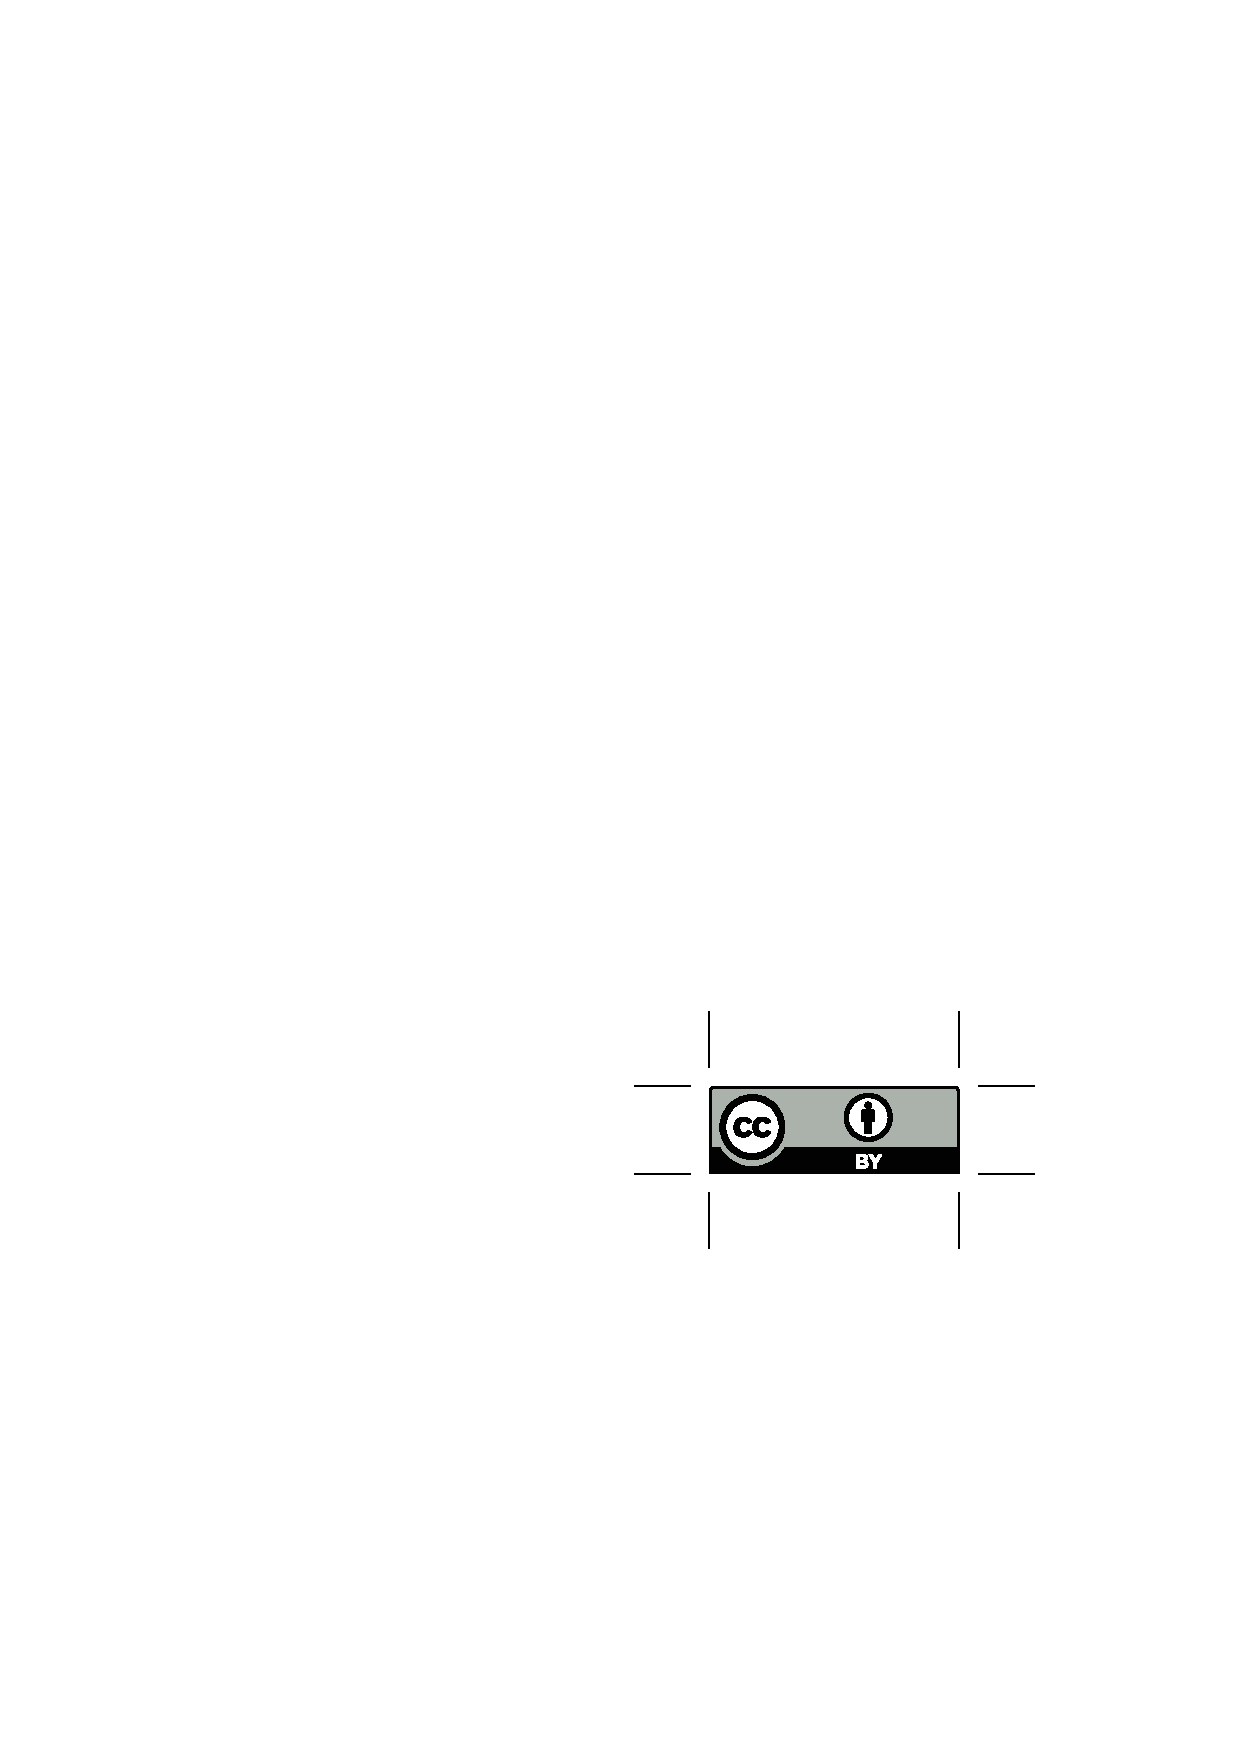
\includegraphics[width=0.90\textwidth]{by}}
  \end{minipage}\hfill
  \begin{minipage}{0.8\columnwidth}
   \href{https://creativecommons.org/licenses/by/4.0/}{This work is licensed under a Creative Commons Attribution International 4.0 License.}
  \end{minipage}
  \vspace{5pt}
}
\makeatother

\setcopyright{ifaamas}
\acmConference[AAMAS 2027]{Proc.\@ of the 26th International Conference
on Autonomous Agents and Multiagent Systems (AAMAS 2027)}{3--7 May 2027}{Hanoi, Vietnam}{M.~Baldoni, F.~Fang, W.~Yeoh, N.~Yorke-Smith (eds.)}
\copyrightyear{2027}
\acmYear{2027}
\acmDOI{}
\acmISBN{}

%%% OpenReview submission number goes here once registered.
\acmSubmissionID{}
\submissionType{Research Paper Track}

\begin{document}

\title{Token-Efficient Context Sharing in Multi-Agent LLM Systems:\\
How Much Can Be Cut, and What Limits It}

\begin{abstract}
Multi-agent LLM systems coordinate by forwarding context between
agents, and every forwarded token is billed. Common practice forwards
whole conversation histories, because deciding what to withhold is
hard, so coordination cost grows quadratically in the number of
agents. We ask a practical question: how much of that traffic can be
removed without paying for it in task quality, and what stops us
removing more?

On a controlled proxy for multi-agent context sharing built from a
public multi-hop benchmark, a $2.7\times$ reduction in inter-agent
tokens produces an uncertain $4.2$-point accuracy loss ($95\%$ CI
$-10$ to $+1$ points): the point estimate favours sending everything,
and the interval does not establish a free region, only that both a
real loss and no loss are compatible with this sample. An oracle
reaches $21\times$ fewer tokens with an observed $+5$-point
\emph{gain}, significant on one of two models tested. Over-delivery
may thus be mildly harmful rather than merely wasteful, with roughly
an order of magnitude available in principle, though the evidence for
that ceiling is directional. A practical policy at $5.4\times$
establishes that a loss exists at that compression, $8$ points with a
CI excluding zero.

\emph{How} the budget is spent matters more than how much is spent.
Allocating per receiver beats selecting one globally-scored set for
everyone by $19.2$ accuracy points at matched cost, and we explain this
with a separation result: the one-set formulation --- the natural
reading of the problem as influence maximization --- loses a factor
$n$ in the number of receivers, by two independent constructions, even
on instances where the objective is monotone and submodular; adding
saturation removes any finite bound. We also show the two nearest
optimisation toolchains do not apply here, the second because its
structural parameters do not exist rather than because its bound is
loose --- and, on the positive side, that the correct per-receiver
formulation costs nothing extra in approximability under an explicit
oracle assumption, since it decomposes exactly into a resource-allocation
program over a shared budget. Abandoning the one-set object is
therefore not a tractability trade.

Finally, a negative result that we think is the most useful finding
for practitioners. None of four value-curve designs fed to a
resource-allocation program that exploits structure no baseline can
showed a detectable advantage over a tuned uniform per-receiver rule
at matched budget, and replacing lexical relevance with a dense
retriever makes matters worse. Three independent lines of evidence
place the binding constraint on \emph{estimating} which agent needs
what, not on the allocation rule.
\end{abstract}

\keywords{multi-agent systems; large language models; communication;
resource allocation; submodular optimization}

\maketitle

\section{Introduction}

A multi-agent LLM system coordinates by passing context. A planner
tells a solver what the constraints are; an auditor is handed the
records it must check. Every such transmission is billed per token, so
coordination is a direct operating cost, and the prevailing
engineering answer --- forward the whole conversation, because
deciding what to withhold is hard and sending everything is safe ---
makes that cost grow quadratically in the number of agents for
architectures that accumulate or broadcast history (sparse topologies
or prefix caching scale differently). We use transmitted tokens as a
proxy for operating cost throughout; real billing also depends on
input/output pricing, caching, and model choice.

This paper treats that as the problem to solve: how much inter-agent
traffic can be removed before task quality suffers, what the
cost--quality frontier's shape is, and what prevents reaching cheaper
allocations.

\paragraph{What we find.} Three things, in decreasing order of how
comfortable they are.

First, \textbf{cutting tokens produces an uncertain, not a zero,
cost}. On a controlled proxy built from a public multi-hop benchmark,
cutting inter-agent tokens by $2.7\times$ has an observed cost of $4.2$
accuracy points (95\% CI $-10$ to $+1$): the point estimate favours
sending everything, and absent a pre-registered non-inferiority test we
do not claim a free region (\S\ref{sec:disc}). An oracle allocation ---
which knows which item each agent needs --- reaches $21\times$ fewer
tokens with an observed $+5$-point \emph{gain}, significant on one of
the two models we test, consistent with LLMs' measured tendency to
degrade under irrelevant
context~\cite{distracted2025,nolima2025,liu2024}. An order of magnitude
is available in principle.

Second, \textbf{how the budget is spent matters more than how much}.
Allocating a possibly different set to each receiver beats choosing one
globally-scored set for everyone by $19.2$ accuracy points at matched
cost. This is not a tuning detail: the one-set formulation provably loses a
factor $n$ in the number of receivers (Proposition~\ref{prop:sep}), by
two independent constructions, on monotone submodular instances; once
saturation is added, the same family admits no finite bound at all.
That formulation is the natural reading of context sharing as
influence maximization~\cite{kempe2003}, so a substantial and
otherwise applicable literature~\cite{borgs2014,tang2015,eim2025} turns
out to optimise the wrong object here. We also show that the nearest general
framework for the messy objective this problem actually has is
unavailable, because its structural parameters fail to exist rather
than merely giving a loose bound (\S\ref{sec:degen}). The switch of
object costs nothing in return: the per-receiver problem decomposes
exactly into a resource-allocation program coupled only by the shared
budget, and any approximation available for one receiver transfers
unchanged to $n$ of them (Corollary~\ref{prop:approx}).

Third, and most useful to anyone building such a system,
\textbf{the remaining order of magnitude is not an optimisation
problem}. We try four value-curve designs in the resource-allocation
program, which exploits separability structure no per-receiver
baseline can imitate, and none beats a tuned uniform per-receiver rule
at matched budget.
Replacing lexical relevance with a dense retriever makes per-receiver
delivery \emph{worse}. Three independent observations converge: the
binding constraint is estimating which agent needs what. In the
composite-receiver design built to expose it (\S\ref{sec:exp}), the
oracle reaches full delivery recall on $208$ tokens where the best
implementable policy reaches only $62\%$ recall on $929$, and no
allocation algorithm closes that gap, because the information required
is absent from the scores rather than badly exploited.

\paragraph{Contributions.} (i) A measured cost--quality frontier for
inter-agent context sharing on a controlled proxy task, including an
uncertain-cost token reduction and the oracle ceiling
(\S\ref{sec:exp}). (ii) A separation result showing the one-set
formulation loses a factor $n$ even on monotone submodular instances
and is unbounded once saturation is added (\S\ref{sec:sep}), with two
degeneracy results removing the standard toolchains
(\S\ref{sec:degen}), including a single instance failing both at once.
(iii) An exact decomposition of the per-receiver problem into a
resource-allocation program coupled only by the shared budget, with
approximability equal to the single-receiver case under an
integer-cost, oracle-access assumption stated precisely
(\S\ref{sec:alg}). (iv) A negative result locating the residual gap in
relevance estimation rather than allocation (\S\ref{sec:exp}). All
theory statements were additionally checked by exhaustive enumeration
on small instances.

\section{Related work}

\paragraph{Influence maximization.} Monotonicity and submodularity of
the spread function license greedy's $(1-1/e)$~\cite{kempe2003}, and
the scaling literature~\cite{borgs2014,tang2015,eim2025} inherits those
assumptions. Recent work relaxes them but keeps the seed-set object:
one chosen set, serving the whole network. Our separation is orthogonal
to the quality of those relaxations.

\paragraph{Non-monotone and non-submodular maximization.} Guarantees
exist for non-monotone submodular
maximization~\cite{feige2011,buchbinder2012}, for weakly submodular
objectives via the sub\-modu\-larity
ratio~\cite{daskempe2011,daskempe2018} or supermodular
degree~\cite{feigeizsak2013}, and for differences of
submodular functions~\cite{iyerbilmes2012}. Closest to our setting,
Shi and Lai~\cite{shilai2024} treat non-monotone, non-submodular
maximization under a knapsack. \S\ref{sec:degen} shows their
parameters do not exist here. Regularized objectives of the form
$g - c$ with $g$ submodular and $c$ modular admit distorted-greedy
guarantees~\cite{harshaw2019}; the density rule we discuss in
\S\ref{sec:alg} is an instance of that lineage, and we credit it as
such rather than presenting it as new.

\paragraph{Context and communication cost in LLM agents.} Empirical
work cuts inter-agent tokens by pruning the message
graph~\cite{agentprune2024}, generating the topology per
task~\cite{gtd2026,todycomm2026}, or sharing key--value caches instead
of text~\cite{kvcomm2026}, none with an optimality guarantee; a survey
of token cost reports no formal treatment of allocation
either~\cite{tokenecon2026}. Closest in spirit, \cite{propagation2025}
finds empirically that intermediate sparsity beats broadcasting,
without an optimization formulation. Closest to our applied setting,
RCR-Router selects a per-agent memory subset under a strict budget, up
to $30\%$ savings, again without guarantees~\cite{rcrrouter2025}. A
parallel line proves guarantees for a \emph{single} receiver: PACMS
treats context assembly as submodular selection~\cite{pacms2026}; BPS
maximizes a monotone submodular benefit minus a modular token penalty,
bicriteria $(1-1/e,1)$, and is the closest prior work~\cite{bps2026}
--- its benefit is a concave, dimension-additive coverage function, so
a pair separately inert but jointly decisive has no representation in
it, the case \S\ref{sec:degen} turns on. \cite{phasetransition2026}
treats finite context windows as hard fan-in limits via a mixing
depth, through majority-vote aggregation rather than set-function
optimization. We are not aware of a formal treatment of multi-receiver
token allocation, nor an influence-maximization framing of LLM-agent
communication.

\section{Model}
\label{sec:model}

Receivers (agents) are indexed $1,\dots,n$. A pool $F$ of information
items is given, item $f$ costing $c(f)>0$ tokens. An
\emph{allocation} assigns a set $S_i \subseteq F$ to each receiver.
Information is copyable, but each transmission is charged, so total
spend is $\sum_i c(S_i)$ and serving $n$ receivers with one set costs
$n$ times serving one. We also consider a \emph{free-broadcast}
convention, where a set may be given to everyone for one transmission,
to show our results do not rest on the cost model.

\begin{definition}[Multi-receiver context allocation]
\label{def:prob}
An instance is a tuple $(n, F, c, (u_i)_{i\le n}, B)$ with $n$
receivers, a finite item pool $F$, a cost $c: F \to \mathbb{R}_{>0}$
extended modularly to sets, per-receiver utilities
$u_i : 2^{F} \to \mathbb{R}$ with $u_i(\emptyset)=0$, and a budget
$B>0$. A feasible \emph{allocation} is a tuple
$(S_1,\dots,S_n) \in (2^{F})^{n}$ with $\sum_i c(S_i) \le B$, and the
objective is $U(S_1,\dots,S_n) = \sum_i u_i(S_i)$. The
\emph{seed-set restriction} of the same instance requires
$S_1 = \dots = S_n$.
\end{definition}

The seed-set restriction is our analogue, in a setting with no
diffusion process, of the commitment an influence-maximization
formulation makes: one chosen set as the entire decision variable.
Classical IM's diffusion can still \emph{reach} different nodes
differently once the seed set is fixed; here, where content is
transmitted directly rather than propagated, the corresponding
restriction is on the delivered content itself, which is why we state
it as a restriction on Definition~\ref{def:prob} rather than import an
IM algorithm unmodified. Fixing everything else in
Definition~\ref{def:prob} and varying only this restriction is what
makes the comparison in \S\ref{sec:sep} a controlled one rather than a
change of subject; \S\ref{sec:exp}'s seed-set baseline is our own
translation of the idea (global top-$k$ by aggregate score) rather
than a published IM algorithm.

Per-receiver utility is
\begin{equation}
u_i(S) = \mathrm{rel}_i(S) - \rho_i\!\left(\mathrm{conf}_i(S)\right),
\label{eq:util}
\end{equation}
relevance minus a saturation penalty, with
$\mathrm{rel}_i(\emptyset)=\mathrm{conf}_i(\emptyset)=\rho_i(0)=0$ so
that $u_i(\emptyset)=0$ as Definition~\ref{def:prob} requires. Two
further features of \eqref{eq:util} are empirically motivated rather
than assumed for convenience. First, $\rho_i$ is increasing: delivering
more context degrades an agent~\cite{distracted2025,nolima2025}.
Second, the penalty's argument is \emph{confusable} load
$\mathrm{conf}_i$, not raw token count, because length-matched studies
find that semantic proximity to the task predicts degradation while raw
length barely does~\cite{liu2024}. Cost and damage are therefore
different quantities in general: one is billed and modular, the other
is semantic and per-receiver; \S\ref{sec:exp} states explicitly where
the experiments collapse this distinction for lack of a confusability
oracle. The objective is $U = \sum_i u_i(S_i)$ subject to the budget.

\begin{example}
Three agents share a pool of $20$ documents. Agent~1 must check a
delivery date, agent~2 a payment total, agent~3 must reconcile the
two. Agents~1 and~2 each need one document; agent~3 needs both. A
uniform allowance of one document per agent starves agent~3; an
allowance of two overfeeds agents~1 and~2 with a document that can
only distract them. No single set serves all three, and the cheapest
correct allocation sends different sets to different agents. This is
the structure Proposition~\ref{prop:sep} makes precise.
\end{example}

\paragraph{Why routing intuitions do not transfer.} The problem is
priced like a delivery problem, which invites a vehicle-routing
analogy that fails on one property: goods are conserved, so a
delivered unit cannot serve a second customer, whereas context is
\emph{copyable} and one item can serve every receiver at once.
Conservation is what makes routing a partition problem; without it,
the allocation is a covering problem, and the interesting constraint
is who should be \emph{spared} an item rather than who gets the last
one. Only \emph{capacity} survives the analogy --- a context window is
rivalrous the way a vehicle is, which is what $\rho_i$ encodes --- and
capacity here is soft, per-receiver, and semantic, so a
per-vehicle-capacity formulation is not a route to the multi-receiver
guarantee we lack.

\paragraph{On the shape of $\rho_i$.} We do not assume $\rho_i$
convex: reported degradation curves are S-shaped, flat then a steep
fall~\cite{nolima2025,liu2024}, and magnitudes are strongly
model-dependent (one study finds large models almost unaffected by
non-confusable filler). Proposition~\ref{prop:decomp} buys the
freedom to avoid that fragility --- the penalty enters only through a
chosen budget level, so $\rho_i$ may be non-convex, discontinuous, or
a cliff. Only the density-greedy \emph{heuristic} of \S\ref{sec:alg},
not the exact dominance test it approximates, needs $\rho_i$
differentiable, and we flag that there as the heuristic's limitation.

\section{Theory: separation, degeneracy, and structure}
\subsection{The seed-set formulation loses a factor $n$}
\label{sec:sep}

\begin{proposition}
\label{prop:sep}
For every $n \ge 1$ there is an instance with $n$ receivers on which,
at an identical budget,
\[
\frac{\mathrm{OPT}_{\text{per-receiver}}}{\mathrm{OPT}_{\text{seed-set}}} = n ,
\]
by two independent constructions: one from the hard budget alone
(cost convention (a) below), one from saturation alone with the
budget non-binding (convention (b)). For every $n \ge 2$, the same
family of instances under convention (b) admits no finite
multiplicative bound at all: the ratio grows without limit as a
distraction penalty $\lambda$ approaches a threshold from below, and
at the threshold $\mathrm{OPT}_{\text{seed-set}}$ is exactly $0$ while
$\mathrm{OPT}_{\text{per-receiver}}$ stays at $n$.
\end{proposition}

\begin{proof}
Take $n$ receivers, $n$ distinct items each of cost $c$, and let
receiver $i$ be satisfied only by item $i$. Set the budget $B = nc$.

\emph{(a) Billed per receiver.} Per-receiver allocation sends item $i$
to receiver $i$, spending $nc = B$ for utility $n$. A seed set $S$
reaches all $n$ receivers and so costs $n|S|c \le nc$, forcing
$|S| \le 1$; a single item satisfies exactly one receiver, for
utility $1$. Ratio $n$.

\emph{(b) Free broadcast, saturating attention.} Let the budget be
non-binding, let a receiver absorb one item freely, and let each
further item cost it $1$. Broadcasting $S$ to everyone yields
$|S| - n\max(0,|S|-1)$, maximized at $|S|=1$ with value $1$, while
per-receiver allocation again yields $n$. Ratio $n$.

\emph{(c) Unboundedness, $n \ge 2$.} Keep the same items and
receivers, keep broadcast free, and let a receiver pay $\lambda \ge 0$
for each item it receives that is irrelevant to it. For a seed set $S$
of size $k$, every item in $S$ satisfies its own receiver and
distracts the other $n-1$, so summing over all $n$ receivers gives
$U_{\text{seed}}(S) = k\bigl(1-\lambda(n-1)\bigr)$, independent of
which $k$ items are chosen. For $0 \le \lambda < 1/(n-1)$ this is
increasing in $k$, so $\mathrm{OPT}_{\text{seed-set}} =
n\bigl(1-\lambda(n-1)\bigr) > 0$ and
\[
\frac{\mathrm{OPT}_{\text{per-receiver}}}{\mathrm{OPT}_{\text{seed-set}}}
= \frac{1}{1-\lambda(n-1)} \;\xrightarrow[\lambda \to (1/(n-1))^{-}]{}\; \infty,
\]
so no $\lambda$-independent finite bound covers this family. At
$\lambda = 1/(n-1)$ the seed-set value is $U_{\text{seed}}(S) = 0$ for
every $S$, so $\mathrm{OPT}_{\text{seed-set}} = 0$; per-receiver
allocation delivers item $i$ to receiver $i$ alone, incurs no penalty,
and attains $n$ regardless of $\lambda$.
\end{proof}

\begin{figure}[t]
\centering
\scalebox{0.8}{%
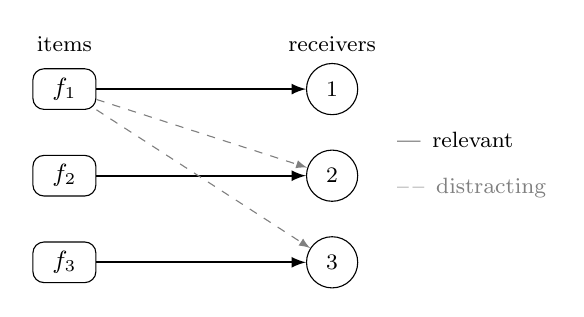
\begin{tikzpicture}[x=1cm,y=1cm,font=\small,
  item/.style={draw,rounded corners,minimum width=8mm,minimum height=5mm},
  recv/.style={draw,circle,inner sep=1.5pt,minimum size=6.5mm}]
\node[anchor=south] at (0,2.55) {\footnotesize items};
\node[anchor=south] at (3.4,2.55) {\footnotesize receivers};
\foreach \i/\y/\lab in {0/2.2/$f_1$,1/1.1/$f_2$,2/0/$f_3$}{
  \node[item] (I\i) at (0,\y) {\lab};
  \node[recv] (R\i) at (3.4,\y) {\footnotesize \the\numexpr\i+1\relax};
}
% relevant edges
\foreach \i in {0,1,2}{ \draw[-latex,thick] (I\i) -- (R\i); }
% distracting edges, drawn only for f_1
\draw[-latex,dashed,gray] (I0) -- (R1);
\draw[-latex,dashed,gray] (I0) -- (R2);
\node[anchor=west,align=left,font=\footnotesize] at (4.05,1.55)
  {\,---\, relevant};
\node[anchor=west,align=left,font=\footnotesize,gray] at (4.05,0.95)
  {\,--\,--\, distracting};
\end{tikzpicture}}
\caption{Proposition~\ref{prop:sep}'s instance at $n=3$: each item is
relevant to one receiver (solid) and distracting to the other $n-1$
(dashed, shown only for $f_1$). Per-receiver follows the solid edges;
a seed set must also send down the dashed ones.}
\label{fig:sep}
\end{figure}

Case (b) is the more informative one. A reader may discount (a) as an
artifact of charging per receiver; (b) removes that objection, because
even with free broadcast the seed set is capped. The reason is worth
stating plainly: \emph{an additional broadcast item helps one receiver
and harms the other $n-1$.}

\begin{remark}
The instance in case (a) contains no saturation and no
complementarity: $\mathrm{rel}$ is modular and $\rho \equiv 0$, so the
objective is monotone and submodular. The separation is therefore not
a consequence of the degeneracies in \S\ref{sec:degen}. Repairing the
objective's curvature does not rescue the seed-set formulation,
because the loss comes from the choice of object, not from the
objective's shape. Any guarantee proved against a seed-set optimum
bounds distance from the wrong quantity.
\end{remark}

Neither construction claims to be the worst case over any class, and
we make no such claim: an instance where every receiver needs the same
item gives ratio $1$ under either convention, so the seed-set loss is
not uniformly $n$ across monotone submodular instances, only
\emph{at least} $n$ on some of them. What (a)--(c) together show is an
existence result on two fronts: the gap is already $n$ on
instances as well-behaved as one could ask (modular relevance, no
saturation, so $U$ is monotone and submodular by
Proposition~\ref{prop:degen}'s own terms), and once saturation is
strong enough to make broadcasting actively harmful, the same family
admits no finite multiplicative bound at all. Both constructions were
checked by exhaustive enumeration over small instances rather than by
algebra alone.

For completeness we record the hardness of the correct object; it is
routine and we claim no credit for it.

\begin{proposition}
\label{prop:hard}
Maximising $U$ subject to $\sum_i c(S_i) \le B$ is NP-hard, already for
$n=1$ and $\rho \equiv 0$.
\end{proposition}

\begin{proof}
With one receiver and no saturation the problem is to choose
$S \subseteq F$ with $c(S) \le B$ maximising a modular $\mathrm{rel}$,
which is \textsc{Knapsack}.
\end{proof}

\begin{remark}
General $n$ does \emph{not} add \textsc{Multiple Knapsack}'s structure
(per-bin capacities, no reuse across bins): here every receiver draws
against \emph{one} shared $B$ and items are copyable, so treating each
receiver-item pair $(i,f)$ as its own object reduces general $n$ (with
$\mathrm{rel}$ modular) to ordinary \textsc{Knapsack} over a larger
ground set --- no harder than $n=1$, consistent with
\S\ref{sec:model}'s point that conservation is what does not transfer.
\end{remark}

\begin{remark}
What Proposition~\ref{prop:hard} does \emph{not} settle is whether
saturation adds hardness beyond the knapsack structure. The
construction above switches $\rho$ off, so the hardness is entirely
attributable to the budget. We leave the question open and note that
Proposition~\ref{prop:approx} below is evidence in the other
direction: the multi-receiver structure adds no approximation hardness
at all.
\end{remark}

\subsection{Both toolchains degenerate}
\label{sec:degen}

\begin{proposition}
\label{prop:degen}
Neither hypothesis of the greedy $(1-1/e)$ argument, nor either
parameter of~\cite{shilai2024}'s general theorem, holds across the
class of Definition~\ref{def:prob}. Precisely, on two separate
witnesses:

\emph{(a) Saturation.} There is an instance with $\mathrm{rel}$
modular and $\rho$ increasing on which $U$ is not monotone, and no
$\gamma_2 \ge 1$ makes $U$ $\gamma_2$-weak supermodular
in the sense of~\cite{shilai2024}.

\emph{(b) Complementarity.} There is an instance --- necessarily with
$\mathrm{rel}$ \emph{not} modular on the receiver where it is
evaluated, since a modular $\mathrm{rel}$ cannot satisfy the
complementarity below --- on which $U$ is not submodular, and no
finite $\gamma_1$ makes $U$ $\gamma_1$-weak submodular.

The two witnesses can in fact be forced simultaneously, on a single
instance: give one receiver (a)'s items and a second, disjoint
receiver (b)'s items. Since neither witness's violating triple
involves the other receiver's items, both violations survive intact
in the combined instance, so no finite $\gamma_1$ \emph{and} no
$\gamma_2\ge1$ exist for it at once. \cite{shilai2024}'s Theorem~4
therefore does not merely fail to cover some instance of
Definition~\ref{def:prob} --- it fails on instances that need only two
receivers.
\end{proposition}

\paragraph{Monotonicity and $\gamma_2$ fail under saturation.} With
$\mathrm{rel}$ modular and $\rho$ increasing, an item whose relevance
falls below its marginal saturation cost strictly lowers $u_i$, so $U$
is not monotone; this is witness (a).

\paragraph{Submodularity and $\gamma_1$ fail under complementarity.}
Two items individually inert but jointly decisive ---
$\mathrm{rel}(\emptyset)=\mathrm{rel}(\{a\})=\mathrm{rel}(\{b\})=0$,
$\mathrm{rel}(\{a,b\})=1$ --- give increasing returns, so $U$ is not
submodular; this is witness (b). Definition~\ref{def:prob} places no
modularity requirement on $\mathrm{rel}_i$, so this instance is a
legitimate member of the class even though it falls outside witness
(a)'s hypothesis. Both failures are required by the greedy argument,
on their respective instances.

\paragraph{The nearest general framework has no parameters here.}
Shi and Lai~\cite{shilai2024} give guarantees for non-monotone,
non-submodular maximization under a knapsack. Their general theorem
requires the objective to be simultaneously $\gamma_1$-weak submodular
and $\gamma_2$-weak supermodular:
\begin{align}
F(U_2 \cup \{x\}) - F(U_2) &\le \gamma_1\left[F(U_1 \cup \{x\}) - F(U_1)\right],
\label{eq:d1}\\
\gamma_2\left(F(U_2 \cup \{x\}) - F(U_2)\right) &\ge F(U_1 \cup \{x\}) - F(U_1),
\label{eq:d2}
\end{align}
for $U_1 \subsetneq U_2$ and $x \notin U_2$. Our two phenomena destroy
exactly one parameter each.

Under complementarity, take the instance above with $U_1 = \emptyset$,
$U_2 = \{b\}$, $x = a$: \eqref{eq:d1} demands $1 \le \gamma_1 \cdot 0$,
which no finite $\gamma_1$ satisfies. Under saturation, an item whose
marginal is $+0.5$ at a lightly loaded receiver and $-1.5$ at a
saturated one makes \eqref{eq:d2} demand
$\gamma_2 \cdot (-1.5) \ge 0.5$, which no $\gamma_2 \ge 1$ satisfies.

\begin{table}[t]
\centering
\caption{Existence of the two parameters that~\cite{shilai2024}
requires \emph{simultaneously}. Each phenomenon destroys exactly one.}
\label{tab:degen}
\begin{tabular}{lcc}
\toprule
 & $\gamma_1$ (weak sub.) & $\gamma_2$ (weak super.) \\
\midrule
Complementarity & \textbf{does not exist} & exists \\
Saturation      & exists & \textbf{does not exist} \\
\bottomrule
\end{tabular}
\end{table}

Table~\ref{tab:degen} summarizes, and the witnesses above --- including
the combined two-receiver instance, checked by exhaustive search over
its whole ground set rather than by algebra alone --- are its proof.
This is a stronger statement than a loose bound: the required
parameters need not exist for instances in the class, not merely take
large values, and a single small instance can lack both at once. It
does not say~\cite{shilai2024} is wrong: its parameters are exactly
right for the class it addresses, most instances of
Definition~\ref{def:prob} (any modular $\mathrm{rel}$ with
$\rho\equiv0$, for one) admit both, and a framework covering ours would
need unbounded local curvature in both directions, which we do not
know how to build. Nor is the result deep: Definition~\ref{def:prob}
places essentially no structure on $\mathrm{rel}_i$, so \emph{some}
instance escaping any fixed finite parameterisation is unsurprising.
What we take from Proposition~\ref{prop:degen} is narrower and, we
think, still useful: saturation and complementarity are two concrete,
independently occurring failure modes, not a claim that this class is
uniquely pathological among unrestricted set functions.

\subsection{Structure and algorithms}
\label{sec:alg}

Proposition~\ref{prop:sep} says the per-receiver object is the right
one. It does not say the resulting problem is intractable, and in one
respect it is unusually well structured.

\begin{proposition}
\label{prop:decomp}
The problem is separable across receivers and coupled only by the
shared budget. Consequently, writing
$v_i(b) = \max\{u_i(S) : c(S) \le b\}$, an optimal allocation is
obtained by solving
\[
\max\Big\{ \textstyle\sum_i v_i(b_i) \;:\; \sum_i b_i \le B \Big\}
\]
and giving receiver $i$ an optimal set at its level $b_i$. If each
$v_i$ is computed exactly, this is exact.
\end{proposition}

\begin{proof}
$U = \sum_i u_i(S_i)$ and the only constraint linking receivers is
$\sum_i c(S_i) \le B$. Fix any feasible allocation and let
$b_i = c(S_i)$. Then $u_i(S_i) \le v_i(b_i)$ and $\sum_i b_i \le B$, so
its value is at most that of the displayed program. Conversely any
feasible $(b_i)$ with maximisers $S_i$ is a feasible allocation of
value $\sum_i v_i(b_i)$.
\end{proof}

Two consequences matter. First, the coupling between receivers is a
single scalar variable, the shared budget $B$, and nothing else --- no
pairwise interaction between receivers survives the reformulation.
Second, and less obviously, the saturation penalty enters \emph{only}
through the chosen level $b_i$, so $\rho_i$ may have any shape
whatever --- non-convex, discontinuous, a cliff. This matters because
the measured degradation curves are S-shaped rather than convex, and a
rule that reasons about $\rho_i'$ requires convexity to argue that its
admission bar rises as a receiver fills.

\begin{remark}
\label{rem:noprice}
The scalar coupling is \emph{not}, in general, a market-clearing
price: that needs every $v_i$ concave, which Proposition~\ref{prop:decomp}
does not assume. Take $v_1(0,1,2)=(0,0,3)$, $v_2(0,1,2)=(0,2,2)$,
$B=2$: the optimum spends all of $B$ on receiver~1, value $3$. For
$\lambda<1.5$ the local optima $\arg\max_b v_i(b)-\lambda b$ sum past
$B$ (infeasible); for $\lambda\ge1.5$ they sum to value at most
$2<3$. No scalar $\lambda$ implements the optimum;
Algorithm~\ref{alg:dp} is exact here precisely because it does not
route through a price. What transfers to every $v_i$, concave or not,
is the reformulation and Corollary~\ref{prop:approx}'s guarantee ---
not a market interpretation of the multiplier.
\end{remark}

The decomposition also yields the one positive guarantee we have. It
says that the difficulty of the multi-receiver problem is concentrated
entirely in the single-receiver subproblems: whatever can be achieved
for one receiver transfers, without loss, to $n$ of them.

\begin{corollary}
\label{prop:approx}
This is a computational oracle in the algorithmic sense, unrelated to
the gold-support policy Table~\ref{tab:policies} calls ``oracle'';
suppose for each receiver $i$ we have one that, given a level
$b$, returns a set $\widetilde{S}_i(b)$ with
$c(\widetilde{S}_i(b)) \le b$ and
$u_i(\widetilde{S}_i(b)) \ge (1-\varepsilon)\,v_i(b)$. Then
Algorithm~\ref{alg:dp}, run on the curves
$\widetilde{v}_i(b) = u_i(\widetilde{S}_i(b))$, returns a feasible
allocation of value at least $(1-\varepsilon)\,\mathrm{OPT}$.
\end{corollary}

\begin{proof}
Let $(b_i^{\star})$ maximise $\sum_i v_i(b_i)$ subject to
$\sum_i b_i \le B$; by Proposition~\ref{prop:decomp} its value is
$\mathrm{OPT}$. The algorithm returns
$\max \{\sum_i \widetilde{v}_i(b_i) : \sum_i b_i \le B\}$, which is at
least $\sum_i \widetilde{v}_i(b_i^{\star}) \ge (1-\varepsilon)\sum_i
v_i(b_i^{\star}) = (1-\varepsilon)\,\mathrm{OPT}$. Feasibility and
attainment hold because each $\widetilde{v}_i(b)$ is realised by an
actual set of cost at most $b$, and $\widetilde{v}_i(b) \ge 0$ since
$\emptyset$ is always available.
\end{proof}

\begin{remark}
The technique is standard resource allocation, credited as such, under
two standing assumptions. Costs are integer, so running time
(Algorithm~\ref{alg:dp}'s table is indexed by $b=0,\dots,B$) is
pseudo-polynomial in $B$, not polynomial in its bit length; and the
oracle hypothesis must hold at \emph{every} level $b$. With
$\rho_i\equiv0$ and $\mathrm{rel}_i$ additionally modular, each $v_i$
is an ordinary knapsack value function with a
$(1-\varepsilon)$-oracle for every $\varepsilon$; for general monotone
submodular $\mathrm{rel}_i$, only $(1-1/e)$ is available, and the
Corollary transfers that coarser ratio instead. Either way the
$n$-receiver problem is no harder to approximate than the
$1$-receiver one: alongside Proposition~\ref{prop:sep}, the seed-set
formulation is off by a factor $n$ or worse while the correct one
costs nothing extra in approximability, so abandoning the one-set
object is not a tractability trade.
\end{remark}

\begin{algorithm}[t]
\caption{Marginal allocation, given any per-receiver oracle}
\label{alg:dp}
\begin{algorithmic}[1]
\Require receivers $1..n$, pool $F$, integer costs, budget $B$, and an
  oracle returning $(V_i(b), S_i(b))$ for every $i,b$ --- exact
  ($V_i{=}v_i$, Proposition~\ref{prop:decomp}) or
  $(1-\varepsilon)$-approximate ($V_i{=}\widetilde{v}_i$,
  Corollary~\ref{prop:approx})
\For{$i = 1$ to $n$}
  \For{$b = 0$ to $B$}
    \State $(V_i(b), S_i(b)) \gets$ oracle$(i, b)$
  \EndFor
\EndFor
\State $A_0(b) \gets 0$ for all $b$
\For{$i = 1$ to $n$}
  \State $A_i(b) \gets \max_{0 \le t \le b}\; A_{i-1}(b-t) + V_i(t)$
  \Comment{for all $b \le B$}
\EndFor
\State recover the levels $(b_i)$ attaining $A_n(B)$
\Return $(S_1(b_1),\dots,S_n(b_n))$
\end{algorithmic}
\end{algorithm}

\begin{example}
\label{ex:dp}
In the running example, $v_1,v_2$ jump from $0$ to $1$ at $b=1$; $v_3$
stays at $0$ until $b=2$, then jumps to $1$. At $B=4$ the DP splits
$(1,1,2)$ for value $3$; a uniform split ($b_i=4/3$, rounding to $1$
each) scores only $2$, wasting a document on agent~3 that it cannot
use alone. A greedy density rule also scores $2$: at the moment it
must choose, agent~3's first document has marginal value $0$ and loses
to agent~1's or agent~2's marginal value $1$, and a zero-marginal item,
once passed over, is never revisited. The DP avoids this because
$v_3$ is built in full before any budget is committed.
\end{example}

Concavifying $v_i$ (time-sharing between two integer levels) does
restore a market-clearing price, but only in \emph{expectation}: if
each receiver randomizes independently, the realized total spend can
exceed $B$ in a given draw even though $\mathbb{E}[\sum_i b_i]=B$.
Exact ex-post feasibility needs the randomization correlated across
receivers (e.g.\ dependent rounding), not independent per-receiver
coin flips; we do not work out that construction here.

The second loop is $O(nB^2)$ arithmetic operations, or $O(nB)$ with the
usual running-maximum bookkeeping when the $v_i$ are concave; either
way it is pseudo-polynomial in the budget and linear in the number of
receivers, so the coupling across receivers is not where the cost
lies. The first loop is the hard part, by
Proposition~\ref{prop:hard}. This is the sense in which the
per-receiver object is well structured: the multi-receiver coupling is
a scalar and the difficulty is local.

Two algorithm families follow, and we are explicit about what is new.

\paragraph{An exact dominance test.} No optimal allocation contains an
item $f \in S_i$ with
\begin{equation}
\Delta\mathrm{rel}_i(f \mid S_i\setminus\{f\}) \;<\;
\rho_i\bigl(\mathrm{conf}_i(S_i)\bigr) - \rho_i\bigl(\mathrm{conf}_i(S_i\setminus\{f\})\bigr).
\label{eq:dominance}
\end{equation}
This is exact, not a first-order approximation: if \eqref{eq:dominance}
holds, deleting $f$ raises $u_i$, because the relevance lost is smaller
than the saturation charge \emph{exactly} avoided, and simultaneously
frees $c(f)>0$ of budget, which can only weaken the constraint. The
resulting allocation is feasible and strictly better, contradicting
optimality, and this needs no assumption on $\rho_i$'s shape --- not
even continuity. It is, however, a condition on the \emph{completed}
$S_i$, checked \emph{ex post}: both sides depend on $S_i$ itself, so it
is a necessary property of an optimum, not a rule for admitting items
one at a time as a set is built. Under complementarity in particular,
an item that fails~\eqref{eq:dominance} against a smaller intermediate
set can satisfy it once the rest of $S_i$ is in place, so a forward
construction that rejects on first failure can discard an item an
optimum would keep.

\paragraph{A density-greedy heuristic.} Building a set that satisfies
\eqref{eq:dominance} still requires deciding an admission \emph{order}.
The standard device, which we credit rather than claim
(distorted-greedy~\cite{harshaw2019}, Algorithm~1
of~\cite{shilai2024}, applied to a single agent with a bicriteria
guarantee by~\cite{bps2026}), ranks candidates by relevance per token,
$\Delta\mathrm{rel}_i(f\mid S)/c(f)$, and admits while a threshold is
cleared. Turning \eqref{eq:dominance} into a per-token threshold
requires relating the exact penalty step to $c(f)$, and this is where
the model's own distinction between billed cost and confusable load
(\S\ref{sec:model}) has to be specialized to say anything operational:
writing $\mathrm{conf}_i(S) := c(S)$ --- confusable load approximated
by token load, for lack of a confusability oracle --- turns
\eqref{eq:dominance} into a same-unit condition on $c(S_i)$, and a
first-order approximation of \emph{that} gives the per-token rule
$\Delta\mathrm{rel}_i(f\mid S)/c(f) \ge \rho_i'(c(S))$ our density-rule
baseline (\S\ref{sec:exp}) implements. Two approximations are stacked
here, not one: the token-load proxy for confusability, and the
first-order step, which additionally needs $\rho_i$ differentiable
where the measured curves are S-shaped. We report the baseline's
results as a heuristic under both approximations, not as an
instantiation of the exact test. A per-receiver threshold, exact or
approximate, also has no view of what a token would buy at another
receiver --- which is exactly what
Algorithm~\ref{alg:dp} adds.

\paragraph{Marginal allocation.} The objective is separable across
receivers and coupled only by the shared budget, so the problem
factors: build each receiver's value-versus-budget curve $v_i(b)$ and
solve $\max \sum_i v_i(b_i)$ subject to $\sum_i b_i \le B$ by dynamic
programming. This equalizes marginal value per token \emph{across}
receivers, which neither a uniform per-receiver rule nor a
per-receiver density rule can do --- the former spends identically on
every receiver, the latter has no view of what a token would buy
elsewhere. The saturation penalty enters only through the chosen
level, so it may take any shape, including the non-convex ones the
measurements suggest. \S\ref{sec:exp} reports that this does not, in
fact, outperform a tuned uniform rule on our benchmark, and why.

\section{Experiments}
\label{sec:exp}

\paragraph{Setup.} We use MuSiQue-Ans~\cite{musique2022}, where the
structure we need is annotated: each instance supplies $20$ candidate
paragraphs with support labels, and sub-questions each carrying the
index of the paragraph answering it. Receivers are sub-questions,
the item pool is the paragraph set, and cost is tokens transmitted
summed over receivers. Ground-truth relevance being labeled makes an
oracle allocation computable. As \S\ref{sec:alg} flags, we take
$\mathrm{conf}_i(S):=c(S)$ throughout, i.e.\ token load stands in for
confusable load; utility is proxied by exact-match accuracy, since
$\mathrm{rel}_i$ and $\rho_i$ are not separately observable outcomes.
Neither substitution is assumed elsewhere: every theory result in
\S\ref{sec:sep}--\S\ref{sec:alg} holds for general $\mathrm{conf}_i$
and $u_i$.

Splitting MuSiQue's single-agent task across per-sub-question receivers
is our framing (\S\ref{sec:disc} discusses this and contamination as
threats to validity); we restrict to the branching families where two
sub-questions carry no back-reference and are genuinely independent.
Comparisons are paired --- every policy answers the same items ---
using McNemar's exact test on discordant pairs and, for the
token--accuracy points, a bootstrap over items.

\paragraph{Protocol.} \texttt{gemini-3.5-flash-lite} (matched-budget
grid) and \texttt{gemini-3.1-flash-lite} (the earlier grid), both at
temperature $0$, called September 2026, sharing one prompt template
(shuffled paragraphs, then the question, ``reply UNKNOWN'' if absent,
answer on a line marked \texttt{ANSWER:}) and one extraction rule (text
after \texttt{ANSWER:}, else the reply's last line), so formatting
cannot differ between policies and arms differ only in which
paragraphs the receiver is given. Lexical relevance is normalized
bag-of-words overlap, $|q\cap t|/\sqrt{|q|\,|t|}$ over non-stopword
tokens; the embedding scorer is \texttt{gemini-embedding-001} at $768$
dimensions, cosine similarity; token counts are word counts scaled by
a fixed constant, not a model tokenizer. $q\in\{0.3,0.7,0.95\}$ are
quantiles of a receiver's own candidate-density distribution
(\S\ref{sec:alg}'s $\mathrm{auto\_scale}$); $k\in\{3,5\}$ are the
cardinalities reported; neither was chosen on a calibration split
disjoint from the evaluation grid --- we do not have one, so we cannot
certify ``tuned uniform'' is free of having been examined on
overlapping data (\S\ref{sec:disc}). The matched-budget grid has $12$
arms over $60$ instances ($1440$ calls, all completed); the earlier
$4$-arm grid covers $69$ instances at $n=138$ receiver-instances ---
both the full branching-family split, no further filtering. Arms are
matched on delivered tokens before accuracy is compared, since an
accuracy gain bought with a larger budget is not a gain from the
mechanism. Runs are keyed and resumable per
$(\text{instance}, \text{policy}, \text{arm}, \text{receiver})$, and
duplicate keys are removed before analysis; without this the pairing
silently breaks and $n$ inflates.

\begin{table}[t]
\centering
\caption{Paired comparisons, $n=120$ receiver-instances ($60$
instances $\times$ $2$ independent sub-questions), matched-budget
grid. $\Delta$ is the first policy minus the second; tokens are each
arm's mean (broadcast $2256$). CI and $p$ are the \emph{primary},
cluster-robust statistics: a block bootstrap and a permutation test
resampling the $60$ source instances, not the $120$ receivers, since
each instance contributes two non-independent receivers --- the flat,
receiver-level version differs negligibly (largest shift: this CI's
lower bound $-.142\to-.150$, $p$ $0.013\to0.028$) and is not shown.
Starred $p<0.05$.}
\label{tab:main}
\footnotesize
\setlength{\tabcolsep}{3pt}
\begin{tabular}{lcccc}
\toprule
Comparison & $\Delta$acc & 95\% CI & $p$ & tokens \\
\midrule
per-r.\ $k{=}3$ (220) vs.\ seed $k{=}3$ (251) & $+0.192$ & $[+.10,+.28]$ & $0.0002^{*}$ & $1.1\times$ \\
oracle (106) vs.\ b'cast & $+0.050$ & $[-.01,+.11]$ & $0.148$      & $21.4\times$ \\
density, loose (846) vs.\ b'cast & $-0.042$ & $[-.10,+.01]$ & $0.225$   & $2.7\times$ \\
unif.\ $k{=}5$ (420) vs.\ b'cast & $-0.083$ & $[-.15,-.03]$ & $0.028^{*}$ & $5.4\times$ \\
density, tight (511) vs.\ unif.\ $k{=}5$ & $+0.000$ & $[-.05,+.05]$ & $1.000$  & $0.8\times$ \\
\bottomrule
\end{tabular}
\end{table}

\begin{table}[t]
\centering
\caption{Accuracy and cost per policy, matched-budget grid, $n=120$.
Tokens are per receiver; the ratio is broadcast's mean tokens divided
by the policy's, from the two numbers shown. Absolute exact-match is
suppressed for deltas since MuSiQue predates current models
(\S\ref{sec:disc}: $0\%$ memorised here, up to $5\%$ on the other
model). ``Density'' is \S\ref{sec:alg}'s density-greedy heuristic (an
approximation of the exact dominance test, \emph{not} an instance of
it) at two thresholds; it is a different policy from
Algorithm~\ref{alg:dp}, evaluated separately in Table~\ref{tab:curves}.}
\label{tab:policies}
\small
\begin{tabular}{lccc}
\toprule
Policy & tokens & ratio & $\Delta$acc \\
\midrule
broadcast (all items)  & $2256$ & $1.0\times$  & --- \\
oracle (labelled)      & $106$  & $21.3\times$ & $+0.050$ \\
per-recv., unif.\ $k{=}3$ & $220$ & $10.3\times$ & $-0.200$ \\
per-recv., unif.\ $k{=}5$ & $420$ & $5.4\times$ & $-0.083$ \\
density, tight $q{=}0.7$ & $511$ & $4.4\times$  & $-0.083$ \\
density, loose $q{=}0.3$ & $846$ & $2.7\times$  & $-0.042$ \\
seed set, $k{=}3$      & $251$  & $9.0\times$  & $-0.392$ \\
random, $k{=}3$        & $336$  & $6.7\times$  & $-0.667$ \\
no context             & $0$    & ---          & $-0.792$ \\
\bottomrule
\end{tabular}
\end{table}

\begin{figure}[t]
\centering
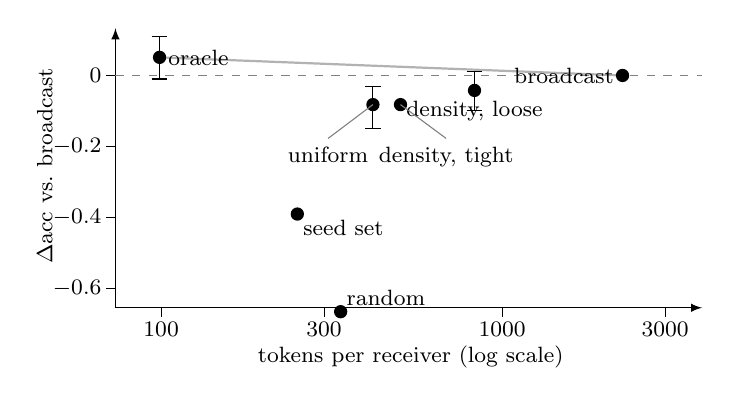
\begin{tikzpicture}[x=1cm,y=1cm,font=\small]
% axes
\draw[-latex] (-0.15,0.2) -- (7.3,0.2);
\draw[-latex] (-0.15,0.2) -- (-0.15,3.75);
% x ticks
\foreach \x/\lab in {0.43/100,2.5/300,4.76/1000,6.83/3000}{
  \draw (\x,0.2) -- (\x,0.08) node[below,inner sep=1.5pt]{\footnotesize\lab};
}
\node at (3.6,-0.42) {\footnotesize tokens per receiver (log scale)};
% y ticks
\foreach \y/\lab in {3.15/{$0$},2.25/{$-0.2$},1.35/{$-0.4$},0.45/{$-0.6$}}{
  \draw (-0.15,\y) -- (-0.27,\y) node[left,inner sep=1.5pt]{\footnotesize\lab};
}
\node[rotate=90] at (-1.05,2.0) {\footnotesize $\Delta$acc vs.\ broadcast};
% broadcast reference line
\draw[dashed,gray] (-0.15,3.15) -- (7.3,3.15);
% frontier: oracle -> broadcast (the achievable envelope)
\draw[thick,gray!60] (0.41,3.38) -- (6.29,3.15);
% points
% 95% CIs (cluster-robust, Table 2) for the three points Table 2 covers
\draw (0.41,3.105) -- (0.41,3.645); \draw (0.31,3.105)--(0.51,3.105); \draw (0.31,3.645)--(0.51,3.645);
\draw (4.41,2.70) -- (4.41,3.195); \draw (4.31,2.70)--(4.51,2.70); \draw (4.31,3.195)--(4.51,3.195);
\draw (3.12,2.475) -- (3.12,3.015); \draw (3.02,2.475)--(3.22,2.475); \draw (3.02,3.015)--(3.22,3.015);
\fill (0.41,3.38) circle (2.4pt);
\node[right,inner sep=3pt] at (0.41,3.38) {\footnotesize oracle};
\fill (6.29,3.15) circle (2.4pt);
\node[left,inner sep=3pt] at (6.29,3.15) {\footnotesize broadcast};
\fill (4.41,2.96) circle (2.4pt);
\node[below,inner sep=2pt] at (4.41,2.9) {\footnotesize density, loose};
\fill (3.12,2.78) circle (2.4pt);
\draw[gray,thin] (3.12,2.78) -- (2.55,2.35);
\node[below,inner sep=2pt] at (2.55,2.32) {\footnotesize uniform};
\fill (3.47,2.78) circle (2.4pt);
\draw[gray,thin] (3.47,2.78) -- (4.05,2.35);
\node[below,inner sep=2pt] at (4.05,2.32) {\footnotesize density, tight};
\fill (2.16,1.39) circle (2.4pt);
\node[below right,inner sep=2pt] at (2.16,1.39) {\footnotesize seed set};
\fill (2.71,0.15) circle (2.4pt);
\node[above right,inner sep=2pt] at (2.71,0.15) {\footnotesize random};
\end{tikzpicture}
\caption{The measured cost--quality frontier, $n=120$
receiver-instances. Vertical bars are $95\%$ cluster-robust CIs for the
three points Table~\ref{tab:main} reports against broadcast (oracle,
density-loose, uniform $k{=}5$); the other points have no CI reported
here. The dashed line is broadcast's accuracy; anything above it is
both cheaper \emph{and} better, though only the oracle's CI clears it.
The implementable policies cluster well below the grey envelope, and
--- the point of the paper's negative result --- they differ from one
another by far less than any of them differs from the oracle. The
seed set at matched cost is $39$ points down, and random delivery
($-0.667$) fixes the scale of the task. An empty-allocation arm (not
shown, $0$ tokens, $-0.792$) is the contamination control.}
\label{fig:frontier}
\end{figure}

\paragraph{The separation appears in the data.} The strongest measured
effect is the first row of Table~\ref{tab:main}: per-receiver
allocation beats a seed-set baseline --- items ranked by aggregate
score and sent to everyone --- by $19.2$ accuracy points at matched
cost. Proposition~\ref{prop:sep} motivates the hypothesis that this gap
grows with the number of receivers --- it is an existence result, not
a prediction about this fused construction, where the candidate pool
and ranking competition also grow with $n$ --- and the hypothesis
holds here: as we fuse instances to raise $n$ from $2$ to $8$ to $16$,
seed-set delivery recall falls from $0.45$ to $0.08$ to $0.01$ while
per-receiver recall stays above $0.55$.

\begin{table}[t]
\centering
\caption{The seed-set gap, motivated by Proposition~\ref{prop:sep} but
not implied by it for this fused construction, grows with the number
of receivers. Delivery recall as instances are fused to raise $n$. The
seed set collapses; per-receiver allocation does not.}
\label{tab:scaling}
\begin{tabular}{lccc}
\toprule
receivers $n$ & $2$ & $8$ & $16$ \\
\midrule
seed set (matched cost)   & $0.45$ & $0.08$ & $0.01$ \\
per-receiver, uniform     & $0.67$ & $0.56$ & $0.56$ \\
\bottomrule
\end{tabular}
\end{table}

\paragraph{A cost--quality frontier, honestly reported.} The loose
density rule cuts tokens $2.7\times$ at an observed, uncertain
$-4.2$-point loss, $95\%$ CI $[-10,+1]$ points (row 3): the point
estimate favours broadcast, and most of the interval is negative, so
this does not establish a free region --- only that a loss up to $10$
points and a loss of zero are both compatible with the data. We report
the estimate and interval rather than a verdict; we did not run a
pre-registered non-inferiority test. Pushing to $5.4\times$ establishes
that a loss exists at that stronger compression, $8.3$ points with a
CI excluding zero (row 4); it does not by itself trace the frontier's
shape between the two points. The oracle beats broadcast by an observed $\sim5$
points at $21\times$ fewer tokens, consistently in sign across two
models ($+0.051$ and $+0.050$) but with a CI excluding zero on only
one of them --- a consistent effect at borderline power, not an
established one.

\paragraph{A negative result on algorithm design.} Across four
value-curve designs, marginal allocation does not beat a tuned uniform
per-receiver rule at matched budget; nor does the density rule
(row 5, exactly zero at $p=1.000$ while spending $25\%$ more). We also found that replacing lexical relevance with one (unnamed)
dense embedding scorer makes per-receiver retrieval \emph{worse}
($0.43 \to 0.25$ top-$1$ recall) while nearly doubling seed-set recall
--- a suggestive contrast we discuss below, not yet a causal one.

\begin{table}[t]
\centering
\caption{Four designs for the value curve $v_i(b)$ that
Algorithm~\ref{alg:dp} consumes, scored by delivery recall at matched
spend against a tuned uniform per-receiver rule, $n=130$ composite
instances (SE~$\approx\!0.04$ on a recall near $0.6$, comparable to
the differences below --- read ``ties'' as \emph{not detectably
different}, not \emph{proven equal}). The structure
Proposition~\ref{prop:decomp} exposes is real; on this benchmark it is
not \emph{estimable}.}
\label{tab:curves}
\begin{tabular}{p{3.9cm}p{3.6cm}}
\toprule
Value curve $v_i(b)$ & Outcome vs.\ tuned uniform \\
\midrule
sum of relevance scores & \textbf{loses}: near-linear in $b$, nothing
to balance \\
noisy-OR over scores & ties; $+4$--$5$pp at large budgets only \\
captured own score mass & ties \\
any of the above, composite receivers & ties ($\approx 11\%$ cheaper
at equal recall) \\
\bottomrule
\end{tabular}
\end{table}

Composite receivers --- a third receiver added to each of $130$
branching instances from the same pool as the two grids above, holding
the instance's full multi-hop question, which needs \emph{all} its
supporting paragraphs where a sub-question receiver needs one ---
manufacture the heterogeneity Proposition~\ref{prop:sep} draws its
advantage from, so a global $k$ must starve one receiver or overfeed
the other. Even then, marginal allocation only matches
uniform, because it can only help where per-receiver value curves are
\emph{distinguishable from label-free signals}, and here they are not:
every receiver draws from a common pool with a similar score
distribution, so an equal split is already near optimal. Heterogeneity
in what receivers \emph{need} did not surface as heterogeneity in what
could be \emph{estimated} about them.

\begin{table}[t]
\centering
\caption{Replacing lexical relevance with a dense embedding scorer
\emph{harms} per-receiver retrieval but helps the seed set. The two
signals fail in opposite directions: embeddings capture what an
instance is about, lexical matching captures which receiver needs
what.}
\label{tab:scorer}
\begin{tabular}{lcc}
\toprule
Delivery recall & lexical & embedding \\
\midrule
per-receiver, top-$1$ & $\mathbf{0.43}$ & $0.25$ \\
per-receiver, top-$5$ & $\mathbf{0.79}$ & $0.61$ \\
seed set, $k{=}3$     & $0.45$ & $\mathbf{0.85}$ \\
\bottomrule
\end{tabular}
\end{table}

A plausible direction for that failure is suggested by the data, on
one unnamed embedding model, so we hold it as a hypothesis rather than
a demonstrated cause. MuSiQue's branching sub-questions are mostly
terse relation templates --- of the form
\texttt{"<entity> >> <relation>"}, for instance
\texttt{"The Poor Boob >> screenwriter"} --- and not natural-language
questions, and exact entity-token overlap locates the right paragraph
directly. The seed-set row of Table~\ref{tab:scorer} is a suggestive,
not causal, contrast: it moves the other way, $0.45 \to 0.85$, since
sending one global set to everyone needs only instance-level
topicality. Embeddings and lexical overlap thus fail in opposite
directions on this benchmark --- one seems to capture what an instance
is about but not who needs what, the other the reverse --- and we
hypothesize that part of the residual gap arises from query
representation rather than scorer family; a hybrid or entity-aware
scorer, and a named, varied set of retrievers (BM25, dense, hybrid), is
the obvious next attempt. We have not tried it, and confirming the
hypothesis needs that intervention, not this single comparison.

Figure~\ref{fig:frontier} puts all of this on one axis. The visual
summary is the paper's argument in miniature: the gap between the
implementable policies and the oracle dwarfs the gaps among the
policies themselves, which is what it looks like when the binding
constraint is not the allocation rule.

Three independent observations thus point the same way: the binding
constraint is relevance \emph{estimation}, not allocation
\emph{optimization}. On the composite-receiver design just described,
the oracle fixes the scale of it, reaching full delivery recall on
$208$ tokens where the best implementable policy reaches only $62\%$
recall on $929$ --- a different sample and metric from
Table~\ref{tab:policies}'s accuracy grid, and not directly comparable
to its $106$-versus-broadcast tokens. No allocation algorithm closes
this gap, because the information required is not present in the
scores.

\paragraph{Logged traces.} Two individual calls from the matched-budget
grid, tracing an over-delivery failure and a seed-set failure item by
item down to the model's own answer, are in the supplementary material
rather than here, to leave room for the analyses above.

\section{Discussion and conclusion}
\subsection{Discussion}
\label{sec:disc}

The results divide cleanly. The formulation-level claims are strong:
the seed-set object is wrong by a factor $n$ on monotone submodular
instances, unboundedly wrong once saturation is added, and both the
classical toolchain and its nearest general successor are unavailable
here. The algorithm-level claims are deliberately weak: no tested
method beats a tuned uniform per-receiver rule, and we report that
rather than a favorable budget point --- a negative result we take as
informative (\S\ref{sec:exp}: heterogeneity in what receivers
\emph{need} did not surface as heterogeneity in what could be
\emph{estimated} here). Genuinely different, predictable appetites are
where the separation's practical value should be sought.

\paragraph{Threats to validity.} We list these in the order we think a
referee should weigh them.

\emph{The multi-receiver framing is ours.} Splitting MuSiQue into
per-sub-question receivers is defensible --- sub-questions and
supporting paragraphs are annotated, which is what makes the oracle
computable --- but no conclusion here measures a deployed multi-agent
system; we restrict to branching decompositions since sequential ones
would make receivers dependent.

\emph{Contamination.} The benchmark predates current models: $0\%$ of
receiver-instances in Table~\ref{tab:policies}'s run are answered
correctly with no context, rising to $5\%$ on the $n{=}138$ grid. We
report policy deltas, not absolute exact-match, so memorisation cannot
be mistaken for policy quality if it affects arms equally.

\emph{Statistical power and clustering.} The oracle-over-broadcast
effect is $+0.051$ on one model, $+0.050$ on the other, significant on
only one ($p=0.039$ vs.\ $0.146$) --- a consistent $\sim5$-point effect
at borderline power. Each original instance also contributes two
receivers sharing a pool and difficulty, so Table~\ref{tab:main}
resamples and permutes at the instance level throughout; the
unreported receiver-level version differs negligibly (three of five
rows unchanged to three decimals, largest shift $p{:}\,0.013\to0.028$),
so this cluster size's design effect is real but small here.

\emph{Calibration of $\rho$.} The saturation penalty's shape comes from
published degradation curves whose magnitude is model- and
task-dependent, and at least one study finds large models unaffected
by non-confusable filler. Proposition~\ref{prop:sep}(a) needs no
degradation at all; the over-delivery claim is only as general as that
literature.

\paragraph{Open problems.} (i)~An unconditional approximation guarantee
for non-trivial $\rho_i$ (Corollary~\ref{prop:approx} reduces this to
the non-monotone, non-submodular single-receiver case), and whether
saturation adds hardness beyond Proposition~\ref{prop:hard}'s knapsack
structure. (ii)~Bundle identification: our witness assumes the
jointly-decisive pair is known, not discovered. (iii)~An end-to-end
multi-agent task on a dependent graph, against stronger receiver-aware
baselines than our global-top-$k$ seed-set translation. (iv)~Endogeneity:
a deployed orchestrator decides which agents to instantiate per task,
with no competitive-analysis treatment that does not first fix a model
of that response.

\subsection{Conclusion}

On a controlled proxy, not a deployed multi-agent system, a
$2.7\times$ reduction produced an uncertain $4.2$-point loss (95\% CI
$-10$ to $+1$), and an oracle reached $21\times$ with an observed gain
--- a ceiling plausibly an order of magnitude, not yet shown free in
between. The obstruction is not degradation or item interaction (both
occur) but that the seed-set object is off by a factor $n$ from the
per-receiver one on well-behaved instances, unboundedly once saturation
is added, at no cost in approximability. That gap runs through better
estimates of what a receiver needs, not better allocation algorithms:
switch to per-receiver allocation, worth $19$ points over the
globally-scored alternative, then spend further effort on retrieval.

\balance
\bibliographystyle{ACM-Reference-Format}
\bibliography{references}

\end{document}
